\documentclass{article}
\usepackage{amsmath} % equation, align, matrix, *, &, \\, \left, \right
\usepackage{graphicx} % figure
\usepackage{subcaption} % subfigure
\usepackage{comment} % To comment
\usepackage{hyperref} % To hyperlink and ref
\usepackage{enumitem} % To list
%\usepackage[ngerman]{babel}
\usepackage[utf8]{inputenc}
\usepackage{wrapfig}
\usepackage{ulem}
\usepackage[backend=bibtex,style=numeric]{biblatex}
\usepackage{subfiles} %multifile latex projects
\usepackage{multirow}
\usepackage{booktabs}
\usepackage{csquotes}
\usepackage[section]{placeins}
\usepackage{color,soul}

%\usepackage{fontspec}
\graphicspath{{images/}{../images/}}

\bibliography{lib} 

\title{IoT System Project - Irrigation Sprinkler}
\author{Tim Reiprich, Tegshigzugder Otgonbayar}

\begin{document}

\pagestyle{plain} \pagenumbering{gobble} %hide page numbers

\maketitle
% \section{}
% \subsection{}
% \subsubsection{}

% \paragraph{}
% \subparagraph{}

\newpage

\pagenumbering{arabic} %show page numbers in arabic
\tableofcontents % from the section headings
\newpage

% \listoffigures \listoftables
% \newpage

\section{Introduction}
In the summer season one of the crucial tasks for people in agricultural field is to provide sufficient water to their crops but also not to overwater. Therefore we have chosen to develop an IoT System Project for managing and regulating irrigation sprinklers automatically and smartly. The use case can be also extended to people for residential and industrial usage. 

\section{General description}
In our project we have three main sensors: light sensor, temperature sensor, and distance sensor. Each sensor has an independent function. Furthermore there is a possibility to combine the these sensors for more complex usage.
In the following the independent functions of the sensors are described:
\begin{itemize}
	\item Light sensor: to sense if it is day or night, so that we can decide when to activate the sprinklers
	\item Temperature sensor: to sense how warm the temperature is, so that the sprinklers are distributing water for a longer or shorter time
	\item Distance sensor: to sense if an object such as a door is open or closed, so that the sprinklers turn off e.g. if a person enters the field
\end{itemize}
  
For the development of this project we have mainly used the applications and tools introduced in the course. Due to do the current pandemic we have opted to build the circuit in the online simulator TinkerCAD instead of a physical circuit. This also enabled us easily to work together. The source code is to be found in our github repository /url{https://github.com/ajpqa/iot2}. The hardware scheme is to be found under \url{https://www.tinkercad.com/things/9b2RV6Rs0I2-projectfinal/editel}.

\section{Hardware Scheme}
In this part we will describe our the scheme of our project, which is to be seen in figure \ref{fig:scheme}. It consists of an Arduino Uno which functions as a micro-controller and collects the data of the environment to control the sprinklers. The sensors to collect data are a temperature sensor, a distance sensor and a light sensor. We measure the temperature because the plants need more water if it's warmer and less if the temperature isn't that high. Furthermore the light sensor is used to determine a good day time to water the plants. Preferably it should always happen in the evening or night as there is a higher chance people work there during the day and plants can get \enquote{burned} if there is strong sun light which gets amplified by water drops on the plants. And lastly we use a distance sensor to determine if the door to the greenhouse is open or closed. If it is open there are workers inside which means that the sprinklers have to be turned off. Only after the door is closed the sprinkler can be turned on again.\par 
The last component of the hardware scheme is the ESP8266 Wifi module which is used to send the measured data to a user interface and Google Cloud using the MQTT protocol. Sadly the Tinkercad circuit simulator doesn't support the Arduino library \texttt{PubSubClient.h} which leads to us not being able to test our configuration properly. In theory the provided code should work in a real environment but sadly the limitations of the simulator are to narrow. So we used a python script to simulate sending the data to the MQTT broker, so that our circuit, user interface and evaluation of the data in Google Cloud works but the transmission of the data has to be simulated by us. 
\begin{figure}
    \centering
	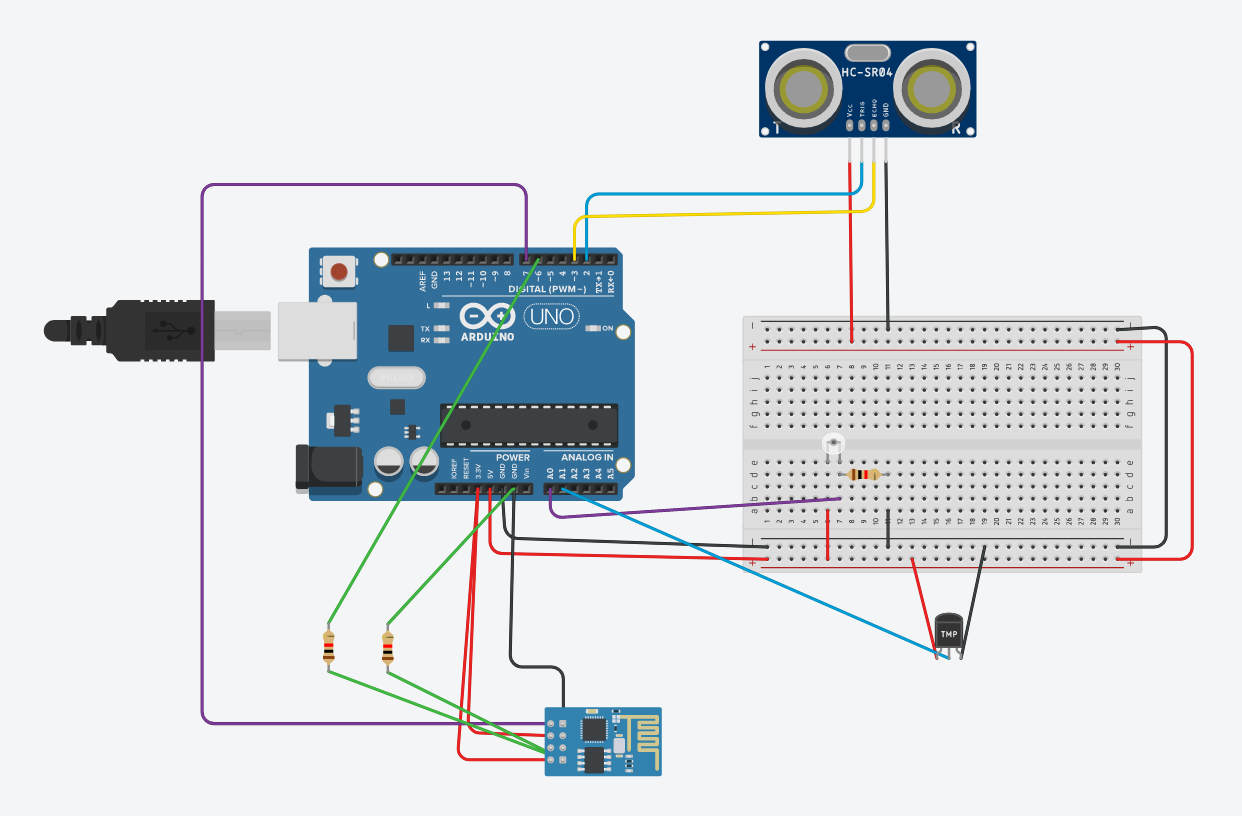
\includegraphics[scale=0.3]{scheme_cropped.png}
	\caption{Circuit that was built during the project}
	\label{fig:scheme}
\end{figure}

\section{Implementation}
The implementation of the project was writtin in the programming languages C++ and Python. The project consists of the following main parts:
\begin{itemize}
    \item project.ino - program for the micro controller
	\item mqtt.py - the mqtt simulation and virtual environment 
	\item main.py - the user interface for the local view and control of sensors and sprinklers
\end{itemize}
\subsection{project.ino}
This file contains the code controlling the Arduino. It's main purpose is to collect the sensor data, convert in humanly standardized measurements and send it via MQTT to a broker. The file can be seen in the Tinkercad project \url{ https://www.tinkercad.com/things/9b2RV6Rs0I2 }.\par 
It consists of multiple functions. Two own helper functions were written. \texttt{sendData} handles sending commands to the ESP8266 Wifi module and \texttt{readUltraSonicDistance} handles measuring the distance as it requires more effort than the other sensors. The two basic functions are \texttt{setup()} and \texttt{loop()}. \texttt{setup()} initializes all variables and sets up the connection to the Wifi while \texttt{loop()} periodically gets the sensors' measurements, prints them to the serial monitor and finally converts the data into a JSON and publishes it via MQTT. Sadly due to restrictions of the Tinkercad simulator the last part can't be used in the simulator as the MQTT library is not available there. Additionally there is a library handling the Wifi connection using the ESP8266 which is also not supported. So we put all the code regarding MQTT and the Wifi library in the file as comments. It should work in a real environment but we couldn't test it as the libraries are just not available. Furthermore we created a python file \texttt{mqtt.py} as a work-around which simulates the publishing of the data (see next chapter).\par
\subsection{mqtt.py}
This is an additional file which would not be needed if we could have used a real circuit but due to the special circumstances we use it to simulate publishing the measured data via MQTT. It simply contains three functions each simulating a sensor and publishes the \enquote{measured} data to the Google Cloud Platform and the hivemind broker where the user interface gets its data from.
\subsection{main.py}
The User Inteface is to be found here. It was mainly created with the widgets of tkinter and tkkinter. It consists of the following three pages; control, value, and summarize.
\paragraph{Control page}
Here is the main control and view of the system. In the "Sensors control" box we can start or stop the receiving of the values of the sensors. In this case depending on a boolean value the received values of the subscription is either inserted or not. In the "Current" values box the most recent received values are shown. The main feature of the distance sensor is to stop the sprinklers in the case that a person or object is moving to the field. In "Automatic Stop" we can set a distance threshold when the trigger object is too close. For example if the object is a door and the door is opened, the sprinkler stops for a period of time until the door is closed again. Here the status is either "Under Threshold" or "Over Threshold". By clicking on the "Confirm" button we can set a new distance threshold.
\begin{figure}
    \centering
	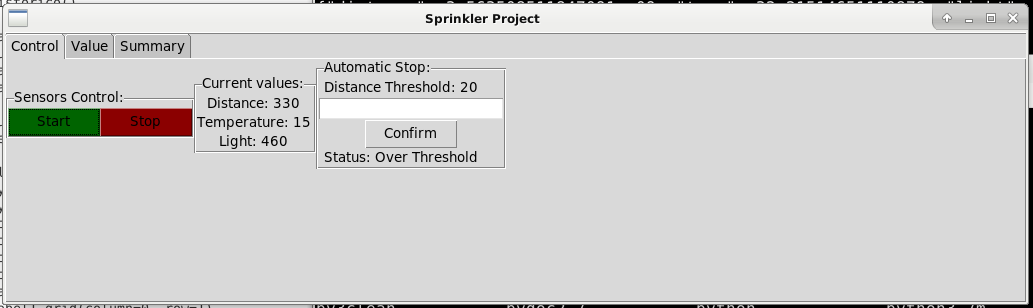
\includegraphics[scale=0.3]{control_view.png}
	\caption{Control Page}
	\label{fig:control}
\end{figure}
\paragraph{Value page}
While in the "Control" page we can only see the most recent values, in the "Value" page all of the values are registered. This can be useful for further analyzing and evaluating based on specific needs of the user. 
\begin{figure}
    \centering
    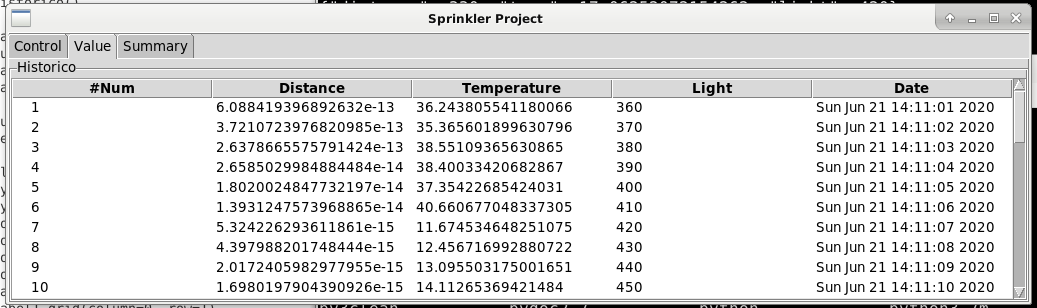
\includegraphics[scale=0.3]{value_view.png}
	\caption{Value page}
	\label{fig:value}
\end{figure}
\paragraph{Summarize page}
The summarize page functions to evaluate the values. With the "Summarize" button the average "temperature" and "light" values are calculated. 
\begin{figure}
     \centering
	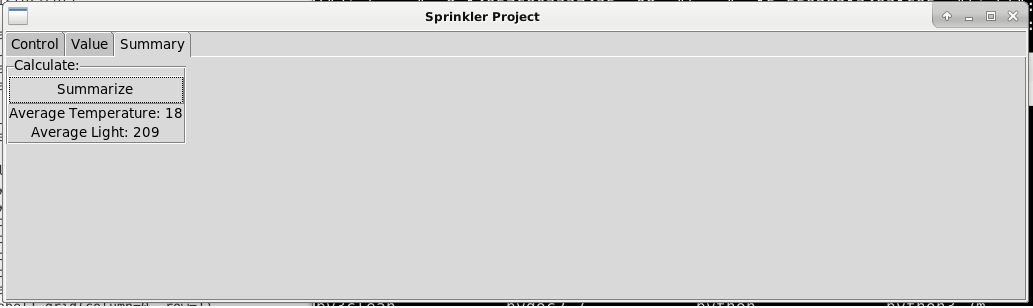
\includegraphics[scale=0.3]{summarize_view.png}
	\caption{Summarize page}
	\label{fig:summarize}
\end{figure}

\section{Google Cloud Platform}
To be able to store the measured data for later analysis we decided to use the Google Cloud Platform as it provides enough storage as well as multiple tools to analyse the stored data.\par 
We used a similar approach like during the classes. We created a new registry and device to receive the data via MQTT using the Pub/Sub tool privided by the Google Cloud Platform. As seen in figure \ref{pic:messages} the data is received successfully.\par 
\begin{figure}
	\centering
	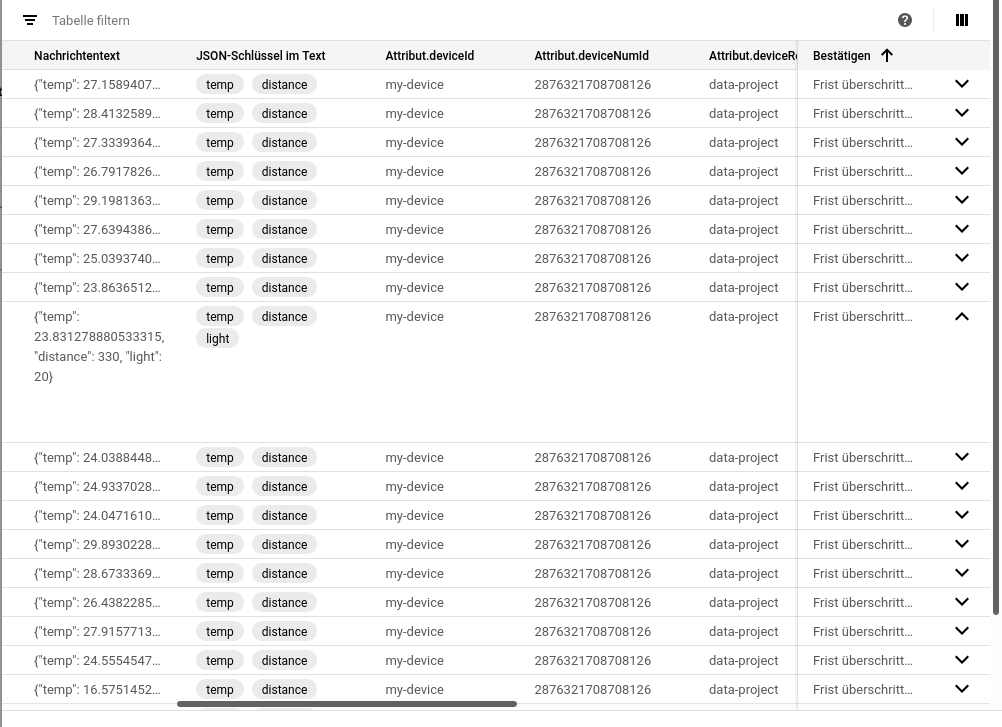
\includegraphics[scale=0.4]{messages.png}
	\caption{received messages via the Pub/Sub tool}
	\label{pic:messages}
\end{figure}
To permanently store the received data we used a Cloud Function to store the data in a SQL table which we created using BigQuery. (see figure \ref{fig:table})
\begin{figure}
	\centering
	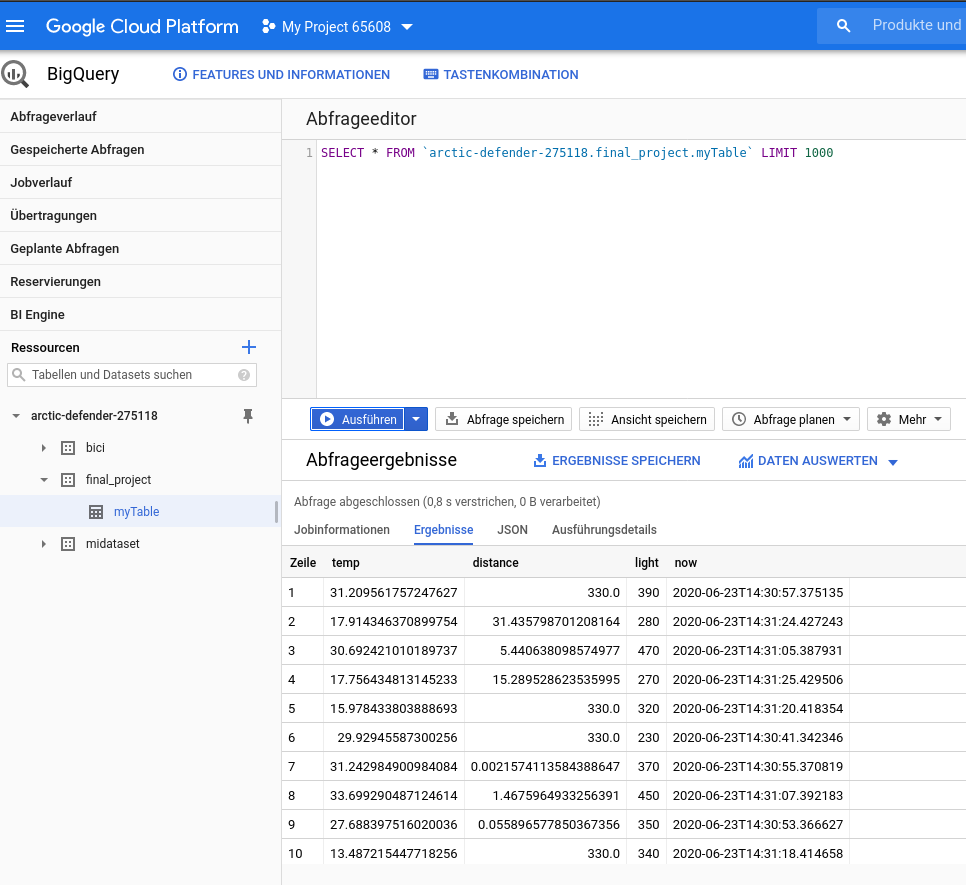
\includegraphics[scale=0.4]{table.png}
	\caption{Stored measurements in a BigQuery table}
	\label{fig:table}
\end{figure}
From there it can be easily extracted to either look at certain data points or analyze it using further tools.
\end{document}
